\begingroup
\newcommand{\GerlingSeptSeconds}[2]{#1\makebox[.42em][c]{,\makebox[0pt][r]{\textsuperscript{s}}}#2}
\begin{center}
\textsc{Gauss} to \textsc{Gerling}.\quad Göttingen, 1~September 1823.
\end{center}

\par\noindent\hspace*{\parindent}\mbox{.\ .\ .\ .\ .\ .\quad I} have merely described my method of telegraphing to you. The numerical signals have no fixed, permanent values, any more than \(a\) and \(x,y,z\) have in algebra. The meanings are always agreed on beforehand for such circumstances as can be anticipated.
I am concerned, however, that telegraphing would be very uncertain, at least with the Meisner heliotrope, for it seems to me that it must be very poorly adjusted.
Particularly in the hour from 2---3\textsuperscript{h} (when the other objects are usually shimmering too strongly for any usable measurement)\textsuperscript{*}), I have invariably found that the light suddenly cuts out at its brightest, then remains completely invisible for a while, gradually reappears as the tiniest point, and only at last reaches full brilliance. Unfortunately, it \textls[120]{retains} that brilliance only for a short time (sometimes only \(\frac{1}{4}\) minute). Under such circumstances, there can be no question of reliable telegraphing.
\par\smallskip\noindent\rule{.24\linewidth}{.4pt}\par\nobreak
{\footnotesize\noindent\hspace*{\parindent}\textsuperscript{*}) Between 6 and 7\textsuperscript{h}, that is, I watched it less often because I did not want to lose any time for measurement.\par}
\smallskip\noindent\hfill{\small49\textsuperscript{*}}\hspace*{.123\linewidth}\par
\clearpage
\noindent\makebox[0pt][l]{\fontsize{13}{16}\selectfont 388}\hfill{\small\textbf{CORRESPONDENCE WITH GERLING.}}\hfill\null\par\medskip
\par\noindent\hspace*{\parindent}In 1822 I had a similar case with the oldest heliotrope, then on the Deister, whose adjustment had presumably suffered from rough transport.
I got around the problem at the time with a temporary remedy.
We made repeated trials. I first indicated to Lieutenant \textsc{Hartmann}, by a particular signal, \textls[120]{that} the trials were to be made.
He then let the image of the sun pass through the crosshairs many times at different heights,
\par\vspace{.7cm}
{\centering
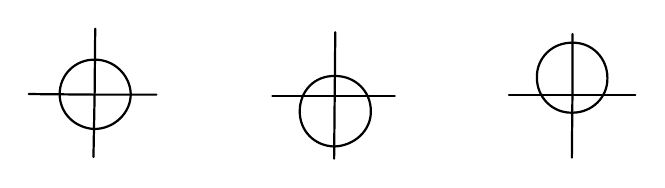
\begin{tikzpicture}[x=.0074cm,y=-.0074cm,line width=.8pt,line cap=round,line join=round]
\draw (103,151) .. controls (103,118) and (130,91) .. (164,92) .. controls (197,92) and (224,119) .. (225,151) .. controls (225,184) and (196,211) .. (162,211) .. controls (129,209) and (103,184) .. (103,151) -- cycle;
\draw (50,151)--(163,152)--(269,152);
\draw (164,39)--(163,151)--(161,259);
\draw (515,181) .. controls (515,146) and (540,119) .. (576,120) .. controls (610,120) and (637,146) .. (637,180) .. controls (638,213) and (609,240) .. (574,241) .. controls (540,240) and (515,214) .. (515,181) -- cycle;
\draw (468,154)--(575,154)--(678,154);
\draw (576,45)--(575,154)--(574,262);
\draw (922,123) .. controls (921,89) and (949,62) .. (983,63) .. controls (1017,62) and (1043,90) .. (1043,123) .. controls (1044,157) and (1016,183) .. (983,183) .. controls (949,184) and (922,157) .. (922,123) -- cycle;
\draw (874,153)--(983,153)--(1091,153);
\draw (983,48)--(983,153)--(982,260);
\end{tikzpicture}\par}
\vspace{.7cm}\noindent and I indicated to him the moment when I first saw his light at full strength by opening my heliotrope, and the end of the light at full strength by covering it.
It goes without saying that the sun was always nearly centred on the crosshairs of my heliotrope during this operation, to make quite sure that my light reached him at full strength.
So 3 people were needed on my side: one to keep the heliotrope nearly centred, a second to observe the heliotrope on the other side through the telescope (the distance was \(8\frac{1}{2}\) miles), and a third to uncover or cover the heliotrope mirror as the second called out (simply by stepping in front of it).
I would very much like to do this with you as well.
The 3-fold attention signal (\GerlingSeptSeconds{1}{2} covered, \GerlingSeptSeconds{1}{2} open, \GerlingSeptSeconds{1}{2} covered, etc.\ etc.) could indicate the intention to make the trial (which one makes only when there is little danger of cloud cover). The first to give the signal is the one who wants to test the other's heliotrope.
Since it is easy to preach to the learned, I need hardly add anything about how to make use of the trials.
With a similar angular setting, this method is almost as good as an actual adjustment, since the person with the heliotrope that was tested knows how to let the sun's image pass through and whether to reset the instrument \textls[120]{before} the sun has passed out of view or after it has already partly passed out of view, etc.
Hopefully the \textls[120]{new} heliotrope will be well adjusted.
\par\noindent\hspace*{\parindent}What you write to me about the \textls[120]{difference} between your signalling and mine is not quite clear to me.
What seems to me absolutely essential
\par\clearpage
\noindent\null\hfill{\small\textbf{ON THE HANOVER TRIANGULATION.}}\hfill\makebox[0pt][r]{\fontsize{13}{16}\selectfont 389}\par\medskip
\noindent is that the attention signal must first be \textls[120]{answered} before the actual signal is given. But whether the former and the latter signals are observed with a separate telescope or, if none is available, with the heliotrope telescope amounts, I think, to the same thing.
\par\noindent\hspace*{\parindent}I have often changed my method of signalling. The one I wrote to you about seems to me the most suitable.
Unfortunately, I neglected to make a copy for myself, and even now I can no longer recall it quite exactly from memory alone.
So please be so kind as to have this passage of my letter \mbox{copied for me.\quad.\ .\ .\ .\ .\ .}
\par
\endgroup
